A partire dalle variazioni di alcuni indicatori relativi al traffico su strada e al traffico aereo, registrate durante il periodo del \textit{lockdown} e descritte nella sezione precedente di questo \textit{report}, sono state stimate le corrispondenti variazioni delle emissioni di alcuni inquinanti in atmosfera.

La base dati di partenza è l'ultima versione disponibile dell'inventario delle emissioni del Friuli Venezia Giulia\footnote{\url{http://www.arpa.fvg.it/cms/tema/aria/pressioni/Catasto_emissioni/catasto.html}}, realizzato da ARPA-FVG con tecnologia INEMAR e riferito all'anno 2013. Dalla base dati sono state escluse alcune emissioni puntuali rilevanti, non attive durante il periodo di studio: la centrale termoelettrica di Monfalcone e l'area a caldo dell'impianto siderurgico di Servola (Trieste).

A partire dalle emissioni totali annuali, le emissioni settimanali in condizioni ``normali'' (cioè in assenza di azioni di contenimento del contagio) sono state calcolate con profili temporali standard.

Le variazioni settimanali degli indicatori di attività registrate nel 2020 sono state considerate rappresentative per tutto il territorio regionale. A partire da esse, le variazioni delle corrispondenti emissioni sono state calcolate con una proporzionalità lineare diretta. Per esempio, la diminuzione del 76\% nei conteggi di veicoli osservata l'ultima settimana di marzo a Pordenone è stata applicata alle emissioni per quella settimana di tutte le aree urbane della regione e di tutte le tipologie di veicoli, a prescindere dal carburante usato e dalla classe veicolare.

Si sono così stimate le variazioni, rispetto alle condizioni attese in assenza delle azioni di contenimento, delle emissioni antropiche regionali in atmosfera. Tali stime di variazione tengono dunque conto solo dei trasporti su strada e del traffico aereo, considerando invece invariate le attività produttive industriali e agricole, i traffici portuali, la produzione energetica e i consumi per il riscaldamento domestico. Tali variazioni potranno essere valutate nei prossimi mesi, quando ulteriori dati saranno disponibili.

L'analisi evidenzia (fig.\ref{fig:riduzioneemissioni}) un calo continuo nelle emissioni tra l'ultima settimana di febbraio e la fine di marzo 2020. Particolarmente marcato il calo delle emissioni di ossidi di azoto (NO\textsubscript{x}), che raggiunge il -25\%, dell'anidride carbonica (CO\textsubscript{2}, -19\%) e del monossido di carbonio (CO, -17\%). Meno netto il calo delle emissioni di polveri sottili (PM10 e PM2.5), inferiore al 10\% e probabilmente almeno in parte compensato dall'aumento nei consumi per riscaldamento domestico a biomassa\footnote{non stimato in questo \textit{report}}. Infine, le emissioni dei composti organici volatili nel loro insieme (COV), di ammoniaca (NH\textsubscript{3}) e di biossido di zolfo (SO\textsubscript{2}) non hanno subito variazioni di rilievo.

Nella prossima sezione si vedrà come a queste riduzioni emissive diversificate corrispondano, anche nelle concentrazioni misurate in aria, effetti differenziati per le varie specie chimiche monitorate.

\begin{figure}
    \centering
    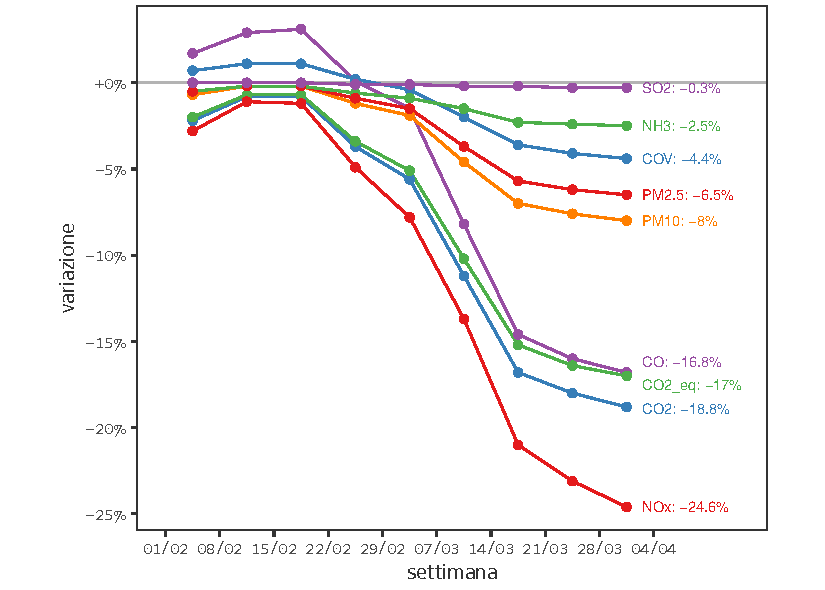
\includegraphics[width=\textwidth]{{figs/riduzioniEmissioni_20200201-20200331}.pdf}
    \caption[Riduzioni delle emissioni antropogeniche]{Riduzioni settimanali delle emissioni antropogeniche delle principali specie chimiche inquinanti e climalteranti in Friuli Venezia Giulia, stimate a partire dagli indicatori disponibili, riferiti al traffico stradale e aereo.}
    \label{fig:riduzioneemissioni}
\end{figure}
